\documentclass[11pt,a4paper]{article}

%==============================================================================%

\usepackage{a4wide}
\usepackage{amsmath,amssymb}
\usepackage[utf8]{inputenc}
\usepackage{float}
\usepackage{graphicx}
\usepackage{listings}
\usepackage{multicol}
\usepackage{tikz}

\usetikzlibrary{arrows}

%==============================================================================%

\newcommand{\assignmentnumber}{7}

\newcommand{\colbreak}{\vfill{\ }\columnbreak}

\newcommand{\modulus}[1]{\left|#1\right|}
\newcommand{\conjugate}[1]{\bar{#1}}
\newcommand{\degree}{^{\circ}}
\newcommand{\limit}[2]{\lim_{#1 \rightarrow #2}}

\newcommand{\figref}[1]{fig. \ref{fig:#1}}
\newcommand{\eqnref}[1]{(\ref{eqn:#1})}

\DeclareMathOperator{\re}{Re}
\DeclareMathOperator{\im}{Im}

\renewcommand\thesection{\assignmentnumber.\arabic{section}}
\renewcommand\thesubsection{\alph{subsection})}

%==============================================================================%

\title{MatIntro Pointopgave \assignmentnumber}
\author
{
    Casper B. Hansen\\
    University of Copenhagen\\
    {\tt fvx507@alumni.ku.dk}
}
\date{\today}

%==============================================================================%

\begin{document}

% \maketitle


% 7.1
\section
{
    \mdseries
    Argumentér for, nedenstående funktion har et maksimum og minimum på den
    angivne mængde. (OBS: Når der ikke anføres "lokalt" eller "globalt", menes
    der per definition "globalt"). Illustrer grafen for funktionen på den
    angivne mængde ved hjælp af Maple. Angiv ud fra figuren, hvad du mener er
    maksimalpunkt og minimalpunkt samt maksimalværdi og minimalværdi.
}
\begin{align}
    f(x,y) &= x + y^2
    \text{,}\quad
    \{(x,y) \in \mathbb{R}^2 | 0 \leq x \leq 2, x - 2 \leq y \leq x\}
\end{align}

\begin{multicols}{2}
    Ved omformulering af ulighederne, som definerer hvilke værdier $x$ hhv. $y$
    kan antage, har vi at $0 \leq x + y^2 \leq 6$, hvilket viser at $f$ er
    defineret i en lukket og begrænset mængde. Dette kan tjekkes efter ved
    $f(0,0) = 0 + 0 = 0$ hhv. $f(2, 2) = 2 + 2^2 = 6$. Af dette kan vi da
    ---jvf. ekstremalsætningen (TLK 2.42)--- slutte, at $f$ har maksimum og
    minimum, og er givet ved uligheden; funktionen $f$ har altså minimalværdi
    $0$ og maksimalværdi $6$.

    Som det fremgår af figuren til højre, er minimalværdien i $f(0,0) = 0$ og
    maksimalværdien i $f(2,2) = 6$.

    \vfill{\ }\colbreak

    \begin{figure}[H]
        \centering
        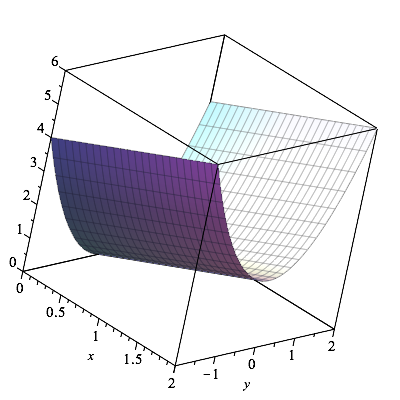
\includegraphics[scale=0.4]{figures/7-1.png}
        \caption{Grafen for $f(x,y) = x + y^2$}
        \label{fig:7-1}
    \end{figure}

\end{multicols}

% 7.2
\section
{
    \mdseries
    Løs TKO 2.17 a) og b) (uden brug af Maple). Derefter skal man ved brug af
    Maple tegne graf og tangentplan i samme figur (altså en figur for hver af
    delopgaverne).
    \\
    Find funktionens tangentplan i det givne punkt.
}

% 7.2 (a)
\subsection
{
    \mdseries $f(x,y) = 1 - 2x + 3y - 4yx$ i ${\bf a} = (1,-1)$.
}
\begin{multicols}{2}
    Lad os bestemme gradienten $\nabla f$. Vi beregner de partielt afledte
    \begin{align}
        \frac{\partial f}{\partial x} = 2 - 4y
        \qquad
        \frac{\partial f}{\partial y} = 3 - 4x
    \end{align}
    og gradienten er dermed
    \begin{align}
        \nabla f(x,y) &= (-2 - 4y, 3 - 4x)
    \end{align}

    Vi kan da beregne tangentplanen
    \begin{align}
        h({\bf x}) &= f(1,-1) + \nabla f(1,-1) \cdot ({\bf x} - a) \\
                   &= (2, -1) \cdot ({\bf x} - a)
                    = 2x - y - 3
    \end{align}

    \colbreak

    \begin{figure}[H]
        \centering
        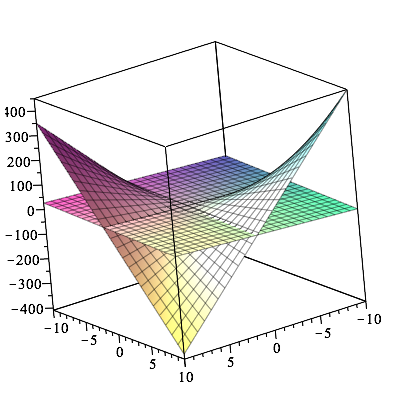
\includegraphics[scale=0.26]{figures/7-2a.png}
        \caption{Tangentplanen for $f$}
        \label{fig:7-2a}
    \end{figure}

\end{multicols}

% 7.2 (b)
\subsection
{
    \mdseries $g(x,y) = \frac{1}{3} x^2 \cos y$ i $b = (\sqrt{3},\frac{\pi}{6})$.
}
\begin{multicols}{2}
    Ligeledes for $g$ beregner vi gradienten $\nabla g$
    \begin{align}
        \frac{\partial g}{\partial x} = \frac{2}{3}x \cos y
        \qquad
        \frac{\partial g}{\partial y} = -\frac{1}{3}x^2 \sin y
    \end{align}
    gradienten er dermed
    \begin{align}
        \nabla g(x,y) &= (\frac{2}{3}x \cos y, -\frac{1}{3}x^2 \sin y)
    \end{align}

    Vi kan da beregne tangentplanen
    \begin{align}
        h({\bf x}) &= g(\sqrt{3}, \frac{\pi}{6})
                    + \nabla f(\sqrt{3}, \frac{\pi}{6})
                      \cdot ({\bf x} - b) \\
                   &= \frac{\sqrt{3}}{2}
                    + \left(
                        \frac{2}{3} \sqrt{3}
                        \cos \left( \frac{\pi}{6} \right),
                        -\frac{1}{3} \sqrt{3}^2 \sin \left( \frac{\pi}{6} \right)
                      \right)
                      \cdot ({\bf x} - b) \\
                   &= \frac{\sqrt{3}}{2}
                    + \left( 1, -\frac{1}{2} \right)
                      \cdot (x - \sqrt{3}, y - \frac{\pi}{6}) \\
                      &= x - \frac{1}{2}y - \frac{\sqrt{3}}{2} + \frac{\pi}{12}
    \end{align}

    \colbreak

    \begin{figure}[H]
        \centering
        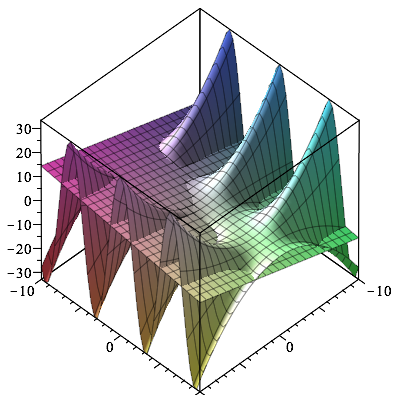
\includegraphics[scale=0.26]{figures/7-2b.png}
        \caption{Tangentplanen for $g$}
        \label{fig:7-2b}
    \end{figure}

\end{multicols}

% 7.3 (ii)
\section
{
    \mdseries
    Tilstandsligningen for (et givet antal mol af) en gas angiver trykket $P$
    som funktion af volumenet $V$ og temperaturen $T: P = f(V,T)$. For en
    idealgas er tilstandsligningen
}
\begin{align}
    P = n R \frac{T}{V}\text{,}
\end{align}
\section*
{
    \mdseries hvor $n$ er moltallet og $R$ er en konstant (gaskonstanten). Man
    kan selvfølgelig også udtrykke volumenet som funktion af tryk og
    temperatur, og temperatur som funktion af tryk og volumen:
}
\begin{align}
    V = n R \frac{T}{P}\text{,} \quad
    T = \frac{PV}{nR}\text{.} \quad
\end{align}
\section*
{
    \mdseries Hvis man (naivt) forkorter i brøkerne, kunne man ledes til at
    tro at produktet
}
\begin{align}
    \frac{\partial P}{\partial T}
    \frac{\partial T}{\partial V}
    \frac{\partial V}{\partial P}
    \label{eqn:partial-prod}
\end{align}
\section*
{
    \mdseries er lig med 1. Dette resultat er imidlertid ikke korrekt.
}
\subsection
{
    \mdseries Beregn ved hjælp af de eksplicitte udtryk ovenfor de partielt
    afledte $\frac{\partial P}{\partial T}$, $\frac{\partial T}{\partial V}$,
    $\frac{\partial V}{\partial P}$.
}
\begin{align}
    \frac{\partial P}{\partial T} n R \frac{T}{V}
    = \frac{n R}{V}
    \qquad
    \frac{\partial T}{\partial V} \frac{P V}{n R}
    = \frac{P}{n R}
\end{align}
\begin{align}
    \frac{\partial V}{\partial P} n R \frac{T}{P}
    = \frac{\partial V}{\partial P} n R T \frac{1}{P}
    = \frac{\partial V}{\partial P} n R T P^{-1}
    = (-1)n R T P^{-2}
    = -\frac{n R T}{P^2}
\end{align}

\subsection
{
    \mdseries Vis at produktet i (\ref{eqn:partial-prod}) er lig med et tal
    forskelligt fra 1, hvilket?
    \\
    Det viser sig, at denne værdi for produktet i (\ref{eqn:partial-prod})
    også holder for mere generelle tilstandsligninger end i idealgasligningen.
}
Vi opstiller, ganger ud og reducerer udtrykket
\begin{align}
    \frac{n R}{V} \cdot \frac{P}{n R} \cdot \left( -\frac{n R T}{P^2} \right)
    = -\frac{n^2 R^2 P T}{n R V P^2}
    = -\frac{n R T}{V P}
    = -n R \frac{T}{V} \cdot \frac{1}{P}
    = - \frac{P}{P}
    = -1
\end{align}

\end{document}
